\documentclass[a4paper,10pt]{beamer}
\usepackage[utf8]{inputenc}
\usepackage{color}
\usepackage{colortbl}
\usepackage{xcolor}
\usepackage{caption}
\usepackage{graphicx}
\usepackage{ragged2e}
\usepackage{hyperref}
\usepackage{marvosym}
\usepackage{mathtools}
\usepackage{mdframed}
\renewcommand{\figurename}{Figura}
\usetheme{Warsaw}

\def\@fnsymbol#1{\ensuremath{\ifcase#1\or \dagger\or \ddagger\or
   \mathsection\or \mathparagraph\or \|\or **\or \dagger\dagger
   \or \ddagger\ddagger \else\@ctrerr\fi}}%
\renewcommand\thefootnote{\fnsymbol{footnote}}   
\renewcommand\thempfootnote{\fnsymbol{mpfootnote}}
\makeatother

%Borra el footer 
\setbeamertemplate{footline}{}

%Enumerar figuras
\setbeamertemplate{caption}[numbered]

%Alternativa a framebreak	
\newcounter{tmp}
\newcommand\savecounter{\setcounter{tmp}{\value{enumi}}}
\newcommand\continuecounter{\setcounter{enumi}{\value{tmp}}}

%Borra cabecera
\setbeamertemplate{headline}{}


\logo{
\includegraphics[scale=0.05]{logoUNAM}}

\begin{document}

\begin{frame}
\Large
\title{Tubos fotomultiplicadores y fotodiodos}
\author{Favio Vázquez}
\date{$1^{ro}$ de septiembre de 2015}

Láminas disponibles en \href{https://github.com/FavioVazquez/DeteccionRayosCosmicos-PCF}{(\color{blue} GitHub})

\maketitle
\end{frame}

\begin{frame}{Índice}

\tableofcontents

\end{frame}

\section{Introducción}
\begin{frame}[allowframebreaks]{Introducción}
\begin{justify}
 El uso masivo de la cuenta de centelladores en la detección y espectroscopia sería 
 imposible sin la disponibilidad de dispositivos que nos permitiera convertir la 
 salida de luz débil de un pulso de centellador, en una señal eléctrica medible. 
 
 \vspace{.3cm}
 
 Los tubos fotomultiplicadores (FM) cumplen con esta tarea muy bien, convirtiendo señales 
 de luz que constan típicamente de no más que unos cientos de fotones, en un pulso 
 de corriente utilizable sin añadir una gran cantidad de ruido aleatorio a la señal.
 
\framebreak

 Existe una gran variedad comercial de estos tubos sensibles a diversas longitudes de onda,
 ultravioleta, luz visible, cercana a la infrarroja y otras del espectro electromagnético.
 
 \vspace{.3cm}
 
 \textbf{Usos}:
 
 \begin{center}
   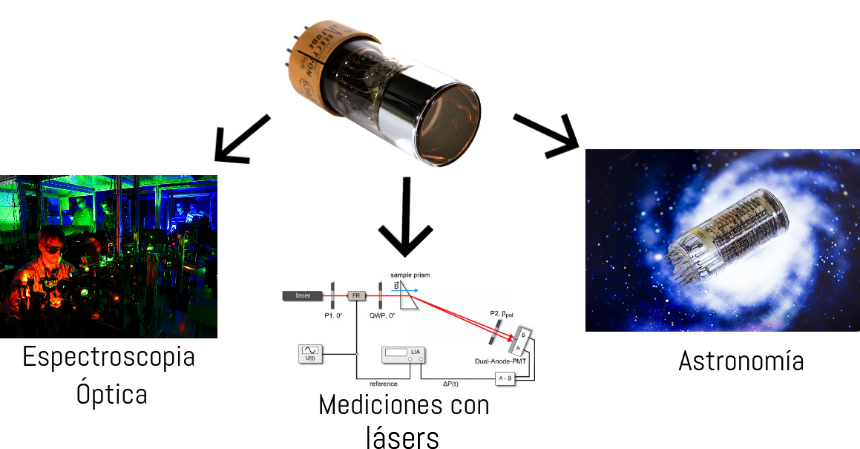
\includegraphics[scale=0.2]{fig1}
 \end{center}

 
 \end{justify}
\end{frame}

\section{Estructura simplificada de un Tubo FM}
\begin{frame}[allowframebreaks]{Estructura simplificada de un Tubo FM}
 
 \begin{columns}[c]
  \column{1.5in}
  \begin{figure}
  \center
   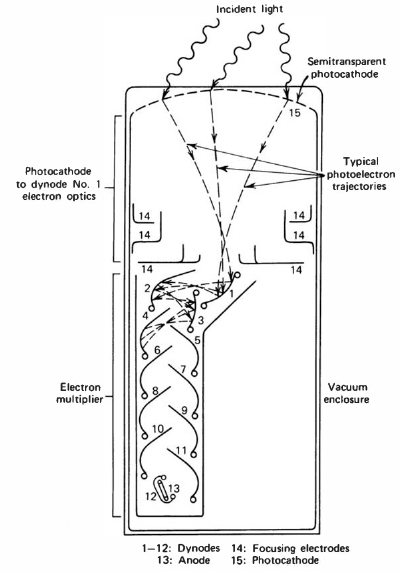
\includegraphics[scale=0.28]{fig2}
   \caption{Elementos básicos de un tubo FM}
  \end{figure}

  \column{2.5in}
  \begin{justify}
   
   \footnotesize{Una envoltura (usualmente de vidrio) sirve como una barrera de presión
   para mantener las condiciones de vacío dentro del tubo, que son requeridas
   para que los electrones de bajas energías puedan ser acelerados eficientemente
   por los campos eléctricos internos.
   
   \vspace{.3cm}
   
   Los dos mayores componentes dentro del tubo son una capa fotosensible, llamada
   el \emph{fotocátodo}, acoplado a una \emph{estructura multiplicadora de fotones}.
   El fotocátodo sirve para convertir la mayor cantidad posible de fotones de luz
   en electrones de baja energía.
   
   \vspace{.3cm}
   
   La sección de multiplicadora de electrones en un tubo FM provee una geometría
   de colección eficiente para los fotoelectrones, y sirve como un amplificador
   casi ideal para incrementar en altas cantidades su número.}
   
   
  \end{justify}

 \end{columns} 
 
 \framebreak
 
  \begin{figure}
  \center
   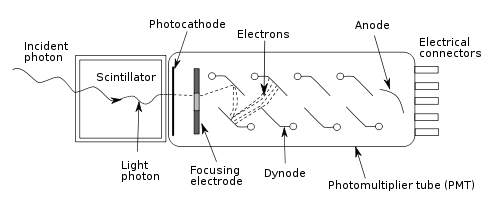
\includegraphics[scale=0.4]{fig3}
   \caption{Elementos básicos de un tubo FM}
  \end{figure}
  
  \begin{justify}
   \footnotesize{
   Luego de una amplificación a través de la estructura multiplicadora, un pulso 
   típico de centellador dará lugar a unos $10^7-10^10$ electrones, suficientes
   para servir de señal de carga para el evento original de centelleo. Esta carga
   es colectada convencionalmente en el ánodo o la etapa de salida de la estructura
   multiplicadora.
   
   \vspace{.3cm}
   
   Tubos típicos, cuando son iluminados por un pulso de luz de muy corta duración,
   producirán un pulso de electrones en un tiempo aproximado de unos pocos nanosegundos
   luego de un tiempo de espera de $20-50$ ns.}
   \end{justify}
    
\end{frame}

\section{El fotocátodo}

\begin{frame}
\begin{center}
 \Huge{\color{blue}El fotocátodo} \\
 \vspace{1cm}
 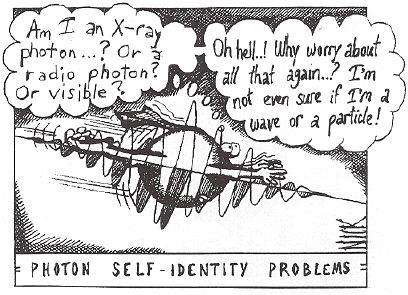
\includegraphics[scale=0.7]{fig4}
\end{center}
\end{frame}


\subsection{El proceso de fotoemisión}
\begin{frame}{El proceso de fotoemisión}
 
 \begin{justify}
  El primer paso realizado por el tubo FM es la conversión de fotones de luz incidente
  en electrones. Este proceso de foto emisión puede pensarse que ocurre en tres etapas
  secuenciales:
  
   \begin{enumerate} [<+->]
  \item La absorción de un fotón incidente y transferencia de energía a un electrón
  dentro del material fotoemisivo,
  \item la migración de ese electrón a la superficie y,
  \item el escape del electrón de la superficie del fotocátodo. 
  \begin{block}{Notas importantes}
  \footnotesize{\begin{justify}La energía que puede transferirse del fotón al electrón en el primer paso está
  dada por la energía cuántica del fotón $hv$ (típicamente $\sim 3$ eV). En el paso 2, alguna de esa energía
  se perderá por las colisiones de electrón-electrón. En el paso 3, debe haber
  la suficiente energía restante para que el electrón pase el potencial barrera
  inherente (\emph{función de trabajo.} (comúnmente $> 3$ o $4$ eV, pero para 
  metales $\sim 1.5-2$ eV)\end{justify}}
 \end{block}
 \end{enumerate}
 
 \end{justify}
  
\end{frame}

\subsection{Emisión espontánea de electrones}
\begin{frame}{Emisión espontánea de electrones}
 \begin{justify}
 La barrera de potencial superficial influencia una propiedad importante de los
 fotocátodos: \emph{el ruido termiónico}. La conducción normal de electrones
 adentro del material del fotocátodo siempre tendrá algo de energía cinética térmica
 que, a temperatura ambiente, se aproximará a los $0.025$ eV. 
 
 \vspace{.3cm}
 
 Si ese electrón está cerca de la superficie, puede escapar y dar lugar a una señal
 inducida térmica espontánea.
  
\begin{block}{Nota relevante}
 \begin{justify}
  En los metales, la tasa de emisión térmica es baja $(\sim 100 \text{m}^2\cdot \text{s})$
  debido a su potencial de barrera relativamente alto. En los semiconductores, el bajo 
  potencial de barrea lleva a tasas de emisión térmicas tan altas como $10^6-10^8 \text{m}^2\cdot \text{s}$
 \end{justify}
 \end{block}
\end{justify}
\end{frame}

\subsection{Fabricación de fotocátodos}
\begin{frame}{Fabricación de fotocátodos}
 \begin{justify}
  
  \small{Los fotocátodos pueden ser construidos tanto por capas opacas o semitransparentes.
  Un fotocátodo opaco es fabricado normalmente con un grosor un poco más grande 
  que la profundidad de escape máxima\footnotemark y es soportado por un material
  de respaldo grueso. Los fotocátodos semitransparentes generalmente no son más 
  gruesos que la profundidad de escape, son depositados en un respaldo transparente 
  (usualmente el final del vidrio del tubo FM).}
  
  \begin{block}{Nota relevante}
  \begin{justify}
   Debido a que son más fácilmente adaptables a diseños de tubo que usan una 
   ventana final plana, los fotocátodos semitransparentes son más comunes en los
   tubos FM diseñados para conteo de centelladores.
   \end{justify}
  \end{block}
  
  \begin{exampleblock}{Nota experimental}
  \begin{justify}
   Las variaciones en el espesor darán lugar a cambios correspondientes en la sensitividad 
   del fotocátodo y pueden ser una fuente de pérdida de resolución en los conteos de 
   centelladores (el problema es $\propto$ al diámetro del tubo).
   \end{justify}
  \end{exampleblock}

  \footnotetext[1]{Profundidad máxima del material, en la que los electrones puedan
  alcanzar la superficie y superar el potencial de barrera.}
  
 \end{justify}

\end{frame}

\subsection{Eficiencia cuántica y respuesta espectral}
\begin{frame}[allowframebreaks]{Eficiencia cuántica y respuesta espectral}
 \begin{justify}
  
  \small{La sensitividad de los fotocátodos se mide comúnmente en el ámbito
  de la física, y con gran significación para el conteo de centelladores
  en términos de la \emph{eficiencia cuántica (EC)} del fotocátodo.
  La eficiencia cuántica se define simplemente como}
  
  \begin{equation}
   EQ = \frac{\text{número de fotoelectrones emitidos}}{\text{número de fotones incidentes}}
  \end{equation}

  \vspace{.2cm}
  
  \small{La eficiencia cuántica sería de $100\%$ para un fotocátodo ideal. Pero
  debido a las limitaciones que les he mencionado, los fotocátodos
  comunes tienen una eficiencia cuántica máxima de $20-30\%$.}
  
  \begin{columns}[c]
    \column{2in}
  \begin{block}{Nota relevante}
  \begin{justify}
   La eficiencia cuántica de cualquier fotocátodo será fuertemente una 
   función de la longitud de onda o la energía cuántica de la luz incidente.
   \end{justify}
  \end{block}
    \column{2in}
  \begin{exampleblock}{Nota experimental}
  \begin{justify}
  Una consideración para seleccionar un fotocátodo es buscar una alta
  eficiencia cuántica sobre el rango de longitudes de onda en el 
  cual el espectro de emisión del centellador es concentrado.
   \end{justify}
  \end{exampleblock}
  \end{columns}

  \pause
  
  \begin{columns}[c]
  \column{2in}
  \begin{figure}
   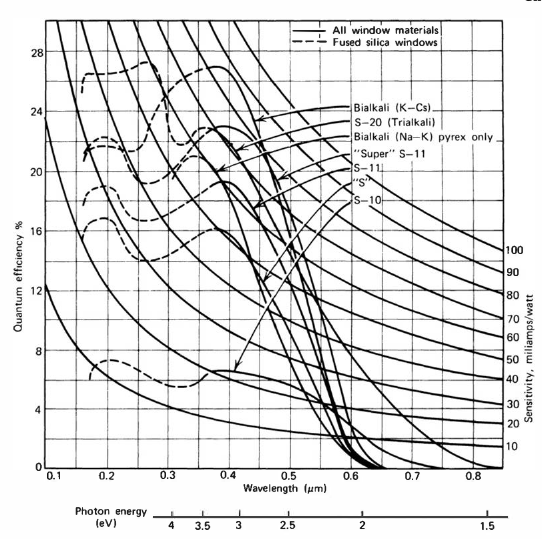
\includegraphics[scale=0.28]{fig5}
   \caption{La eficiencia cuántica es función de la longitud de onda
   o de la energía cuántica de la luz incidente}
  \end{figure}
  
  \column{2in}
  \begin{justify}
  \footnotesize{A una $\lambda$ lo suficientemente alta el electrón no tiene la suficiente
  energía para escapar la superficie del fotocátodo y la respuesta se 
  hace cero. Para vidrio normal, el límite será a $\lambda \sim 350$ nm,
  que es usualmente adecuado para la mayoría de los materiales de centelladores.}
  \end{justify}
  
  \begin{exampleblock}{Nota experimental}
   \begin{justify}
   \footnotesize{Una medida alternativa para la EQ es usada en el conteo de 
   centelladores. Debido al uso extendido de yoduro de sodio 
   activado con talio como cristal de centelleo, se habla de EQ 
   en términos de el número de fotoelectrones producidos por un
   fotocátodo dado por keV de pérdida de energía en un cristal
   de NaI(Tl) para el cual casi toda la luz es colectada.}
   \end{justify}
  \end{exampleblock}

  \end{columns}

  \framebreak
  
  \textbf{Materiales actuales para la construcción de fotocátodos}:
  
  \begin{itemize}
   \item \begin{justify}Materiales multialcalinos basados en el compuesto Na$_2$KSb,
   preparados por activación con una pequeña cantidad de cesio 
   $\Rightarrow$ EQ $\sim 30\%$.\end{justify}
   \item \begin{justify}Materiales bialcalinos basados en K$_2$CsSb activados con
   oxígeno y cesio $\Rightarrow$ $45\%$ a los 350 nm de máxima respuesta.\end{justify}
   \item \begin{justify}Materiales ultrapuros que reducen las trampas de electrones,
   reduciendo reflexiones desde el fotocátodo mediante una introducción
   de de una capa anti-reflejante entre él y la envoltura de vidrio.\end{justify}
   \item \begin{justify}Estructuras prismáticas con un alto radio de superficie 
   a volumen para aumentar la probabilidad de escape de fotoelectrones.\end{justify}
  \end{itemize}

  
 \end{justify}
\end{frame}

\section{Multiplicación de Electrones}

\begin{frame}
\begin{center}
 \Huge{\color{blue}Multiplicación de Electrones} \\
 \vspace{0.5cm}
 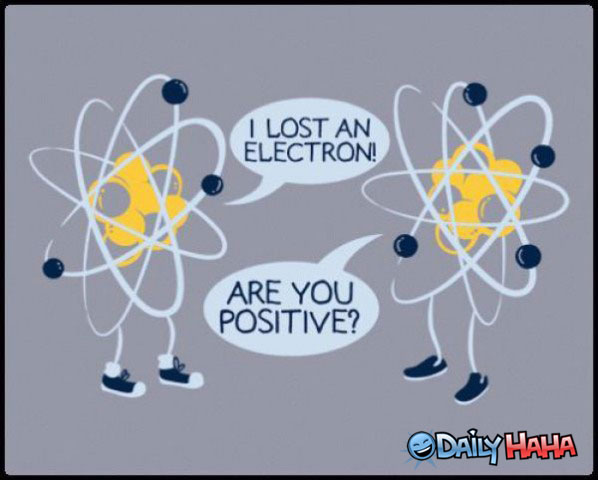
\includegraphics[scale=0.3]{fig6}
\end{center}
\end{frame}

\subsection{Emisión secundaria de electrones}
\begin{frame}{Emisión secundaria de electrones-I}


\begin{columns}[c]

 \column{2in}
\begin{figure}
   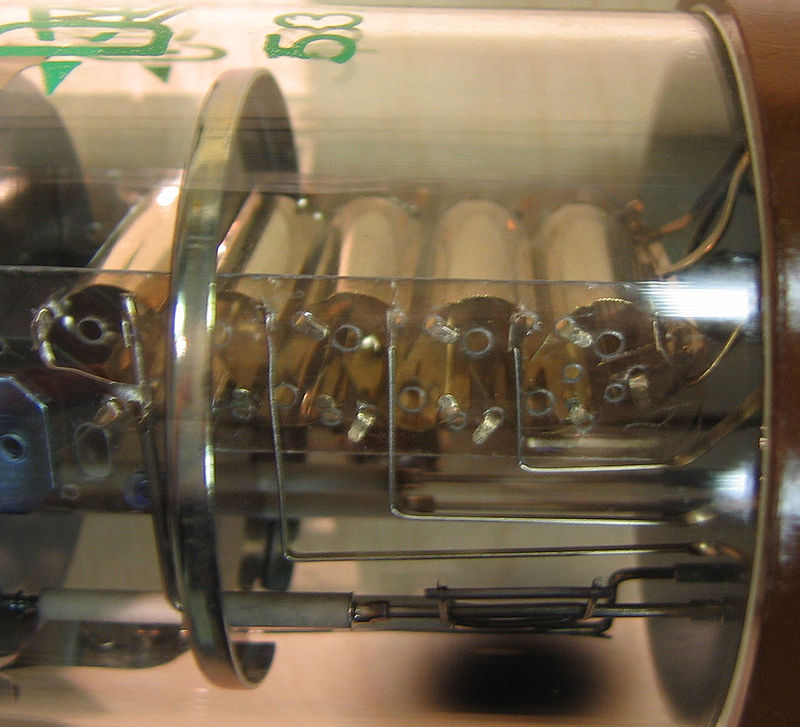
\includegraphics[scale=0.32]{fig7}
   \caption{Dos filas de dínodos dentro de un tubo FM.}
  \end{figure}
  
  \column{2.3in}
\begin{justify}
  Los electrones desde el fotocátodo son acelerados y llevados a chocar la superficie 
  de un electrodo, llamado el \emph{dínodo}. Si el material del dínodo se escoge bien,
  la energía depositada por el electrón incidente puede resultar en la re-emisión de 
  más de un electrón desde la superficie.
 \end{justify}

 \end{columns}

\begin{itemize}[<+->]

 \item[]  \begin{block}{Nota relevante}
  \begin{justify}
  \begin{footnotesize}
   El proceso de emisión secundaria de electrones es similar al proceso que acabamos 
   de ver, pero en este caso los electrones dentro del material del dínodo son 
   exitados por el paso de un electrón energético en vez de un fotón óptico.
   \end{footnotesize}
  \end{justify}
 \end{block}

\end{itemize}
\end{frame}

  
\begin{frame}{Emisión secundaria de electrones-II}

 \begin{footnotesize}Los electrones que dejan el fotocátodo tienen una energía $\sim 1$ eV, o menos. 
 Por lo tanto, si el primer dínodo tiene unos cuantos cientos de voltios positivos, 
 la energía cinética de los electrones al llegar al dínodo está determinanda por 
 el voltaje de aceleración. \end{footnotesize}
 
  \begin{exampleblock}{Nota experimental}
  \begin{footnotesize}
  \begin{itemize}[<+->]
   \item \begin{justify}
          La creación de un electrón excitado en el material del dínodo requiere una
          energía al menos igual a la del bandgap $\sim 2-3$ eV.
         \end{justify}
   \item \begin{justify}
          Es teóricamente posible que para un electrón incidente, se creen un 
          aproximado de 30 electrones exitados por cada 100 V de voltaje acelerador.
         \end{justify}
   \item \begin{justify}
          Debido a que la dirección de estos electrones es aleatoria, (1) algunos 
          no llegarán a la superficie antes de des-excitarse, (2) otros llegan 
          pero han perdido tanta energía que no pueden superar el potencial de barrera
          y no pueden escapar. Por lo que solo una pequeña fracción de electrones 
          excitados contribuirá últimamente a la emisión secundaria dada en la 
          superficie del dínodo.
         \end{justify}
   \item \begin{justify}
          La producción de electrones secundarios es una función sensible a la 
          energía de los electrones incidentes.
         \end{justify}

  \end{itemize}  
  \end{footnotesize}
 \end{exampleblock}
\end{frame}

\begin{frame}[label=milink1]{Emisión secundaria de electrones-III}

\begin{columns}[c]
    \column{2in}
 \begin{figure}
  \center
     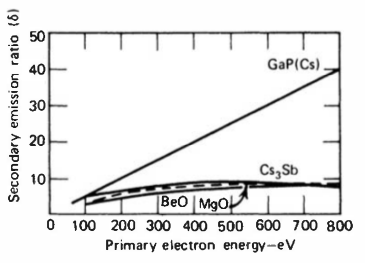
\includegraphics[scale=0.4]{fig8}
     \caption{Variación de la producción en la emisión secundaria con energía 
   de electrón primaria para algunos materias estándares de dínodos (las 
   tres de abajo) y un material NEA (negative-electron affinity) [GaP(CS)]}
   \label{fig:fig8}
   \end{figure}
   \column{2in}
 \begin{block}{Factor de multiplicación}
  El factor de multiplicación para un dínodo está dado por:
  \begin{equation*}  
   \delta=\frac{\text{\parbox{12em}{\center número de electrones secundarios emitidos}}}{\text{electrones primarios
   incidentes}}
  \end{equation*}
  \begin{justify}Este debe ser lo más grande posible para una máxima amplificación por etapa 
  en el tubo FM.
  \end{justify}
  \end{block}
  \end{columns}
\end{frame}


\subsection{Materiales de afinidad electrónica negativa}
\begin{frame}{Materiales de afinidad electrónica negativa - I}

\begin{columns}[c]

\column{2.3in}
\begin{justify}
\begin{footnotesize}
 La producción de emisión secundaria de los dínodos puede ser aumentada significativamente 
 a través del uso de materiales de \textbf{afinidad electrónica negativa} (La afinidad electrónica es la 
 variación de energía que se produce en la adición de un electrón al átomo en estado fundamenta
 y en fase gaseosa para formar el anión correspondiente. La afinidad electrónica puede ser energía desprendida,
 en cuyo caso tiene valor negativo y se trata de átomos con tendencia a captar electrones - no metales.)
 \end{footnotesize}
 \end{justify}
 \column{2in}
 
 \begin{center}
  
\includegraphics[scale=0.2]{fig9}
 \end{center}


\end{columns}
 
  \begin{block}{Nota relevante}
  El más exitoso de estos materiales ha sido el fosfuro de galio (GaP), altamente 
  dopados, a una concentración de casi $10^19$ átomos/cm$^3$ con zinc. Y una capa
  delgada de cesio.
 \end{block}

\end{frame}

\begin{frame}{Materiales de afinidad electrónica negativa - II}

\begin{figure}
 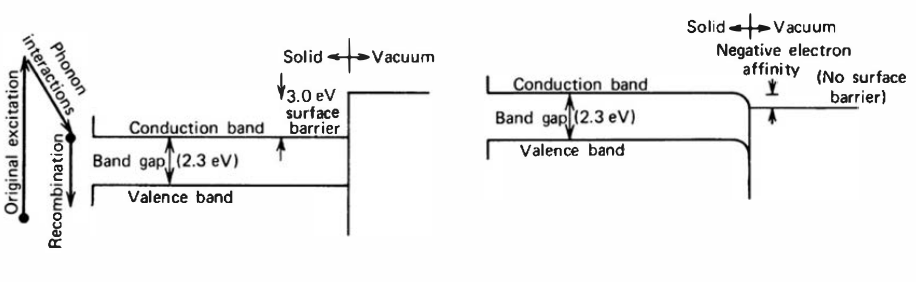
\includegraphics[scale=0.33]{fig10}
 \caption{Estructura de banda cerca de la superficie para semiconductores 
 convencionales (izquierda) y materiales NEA (derecha).}
\end{figure}

\begin{block}{Nota relevante}
\begin{justify}
 A la derecha se muestra la flexión de banda creada por el llenado de lugares 
 aceptadores en la superficie por la capa delgada de Cs. El efecto de esto, 
 es llevar el potencial de vacío más abajo que el del fondo de la banda de 
 conducción en el interior del material.
 \end{justify}
\end{block}

\end{frame}

\begin{frame}{Materiales de afinidad electrónica negativa - III}
 
 \begin{exampleblock}{Nota experimental}
  \begin{itemize}
  \item \begin{justify}
	El efecto neto es que los electrones que han llegado al fondo de la banda 
	de conducción, aún son candidatos a escapar, y se quedan así por un tiempo 100
	veces mayor que antes 
	\end{justify}
 \item \begin{justify}
        Este aumento de tiempo en que los electrones pueden escapar, aumenta 
        las probabilidades de escapa para un electrón típico\footnote{Ver figura
        5. \hyperlink{milink1}{\beamerreturnbutton{Ir}}}.
       \end{justify}
  \end{itemize}
 \end{exampleblock}
 
 \begin{block}{Nota relevante}
  Otra ventaja de utilizar materiales NEA es en tubos FM usados para 
  aplicaciones de medición temporal ultrarápida.
 \end{block}
\end{frame}

\subsection{Múltiples etapas de multiplicación}
\begin{frame}{Múltiples etapas de multiplicación - I}
 \begin{justify}
 Los electrones son guiados por otro campo eléctrico de dínodo en dínodo, en
 la cual se repite la etapa  de multiplicación varias veces. Si se requieren 
 $N$ etapas en la sección multiplicadora, la ganancia total para el tubo FM
 está dada simplemente por 
 
 \begin{equation}
  \text{Ganancia total} = \alpha \delta^N
 \end{equation}
 
 donde $\alpha$ es la fracción de todos los fotoelectrones colectados por la 
 estructura multiplicadora.
\end{justify}
 
 \begin{exampleblock}{Nota experimental}
 \begin{itemize}
 \begin{footnotesize}
\item \begin{justify}
  Los materiales de dínodo convencionales están caracterizados por valores típicos 
  de $\delta=5$ y $\alpha \sim 1$ para tubos bien diseñados. Entonces diez etapas
  resultarán en una ganancia total de $5^10$ o $10^7$. Sise utilizan materiales 
  NEA entonces $\delta \sim 55$, y la misma ganancia se puede conseguir en 4 etapas.
 \end{justify}
\item \begin{justify}
       La ganancia total de un tubo FM es una función sensible del voltaje aplicado $V$.
      \end{justify}
 \end{footnotesize}
 \end{itemize} 
 \end{exampleblock}

 
\end{frame}

\subsection{Estadística de la multiplicación de electrones}
\begin{frame}{Estadística de la multiplicación de electrones - I}

\begin{justify}
 La emisión de electrones secundarios es un proceso estadístico, y por lo tanto el 
 valor específico de $\delta$ en un dínodo dado, fluctuará de evento en evento sobre 
 su valor medio. En el modelo más simple, la producción de electrones secundarios en 
 un dínodo, puede asumirse que sigue un distribución de Poisson sobre la producción media.
 Por lo tanto para un un fotoelectrón incidente en el primer dínodo, el número de 
 secundarios productidos tiene un valor medio de $\delta$ y una desviación estándar 
 $\sigma$ de $\sqrt{\delta}$.
 \end{justify}
 
 \begin{columns}[c]

 \column{2in}
 \begin{block}{Nota Relevante}
 \begin{justify}
 \begin{footnotesize}
 La varianza relativa definida por $(\sigma/\delta)^2$, es igual a $1/\delta$. Recordando 
 la distribución de Poisson, entonces es fácil ver que cuando este proceso se repite 
 sobre $N$ etapas idénticas en el tubo FM, el número medio de electrones colectados en 
 el ánodo será igual a $\delta^N$.
 \end{footnotesize}
 \end{justify}
 \end{block}
 \column{2in}
 \begin{block}{Nota Relevante}
 \begin{justify}
  Si $\delta \gg 1$, entonces la varianza relativa o la expansión en la amplitud 
  del pulso de salida es dominada por fluctuaciones en la producción desde el primer
  dínodo, donde el número absoluto de electrones es el más pequeño.
  \end{justify}
 \end{block}
 \end{columns}

\end{frame}

\begin{frame}{Estadística de la multiplicación de electrones - II}
 \begin{columns}[c]
  
  \column{1.5in}
\begin{figure}
 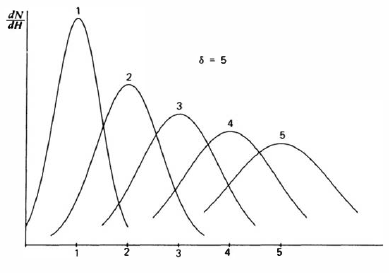
\includegraphics[scale=0.35]{fig11}
\end{figure}
  \column{1.5in}
\begin{figure}
 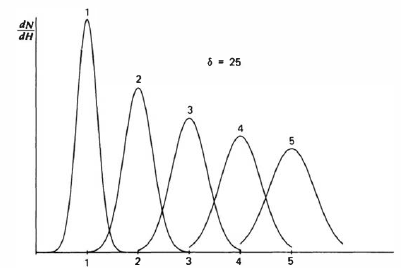
\includegraphics[scale=0.35]{fig12}
\end{figure} 
 \end{columns}
 
 \begin{exampleblock}{Nota experimental}
  \begin{justify}
  \begin{footnotesize}
   Las figuras de arriba muestran la distribución esperada en el número de 
   electrones secundarios producidos por el primer dínodo, cuando es golpeado 
   por diferentes números de fotoelectrones. Si el valor de $\delta$ es pequeño 
   es imposible separar limpiamente los eventos causados por un fotoelectrón de 
   aquellos en los que más fotoelectrones están presentes.
   \end{footnotesize}
   \end{justify}
 \end{exampleblock}
\end{frame}

\begin{frame}{Estadística de la multiplicación de electrones - III}

 \begin{columns}[c]
 
\column{2in}

\begin{figure}
 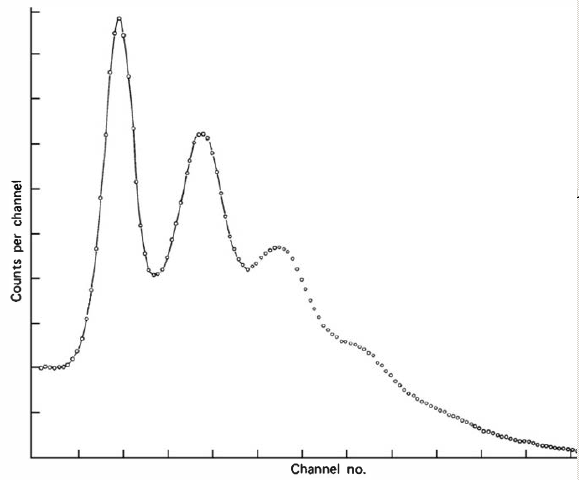
\includegraphics[scale=0.2]{fig13}
\end{figure}

\begin{exampleblock}{Nota experimental}
\begin{justify}
\begin{footnotesize}
Si los dínodos están caracterizados por valores grandes de $\delta$, la separación 
es mucho más discernible y es posible distinguir picos en la distribución correspondiente 
a números discretos de fotoelectrones hasta 4 o 5.
\end{footnotesize}
\end{justify}
\end{exampleblock}

\column{2in}

\begin{exampleblock}{Nota experimental}
\begin{justify}
\begin{footnotesize}
Algunas mediciones experimentales muestran una varianza relativa mayor que la predicha 
por el modelo de Poisson. De hecho, algunas observaciones no muestran picos, sino 
una distribución tipo exponencial. Esto ha llevado a utilizar modelos de distribución
Polya, Poisson compuestos y algunos otros. \textbf{No existe aún una descripción universal
que acomode todas las mediciones experimentales en este caso.}
\end{footnotesize}
\end{justify}
\end{exampleblock}

\end{columns}

\end{frame}

\section{Características de los tubos FM}

\begin{frame}
\begin{center}
 \Huge{\color{blue}Características de los tubos FM} \\
 \vspace{0.5cm}
 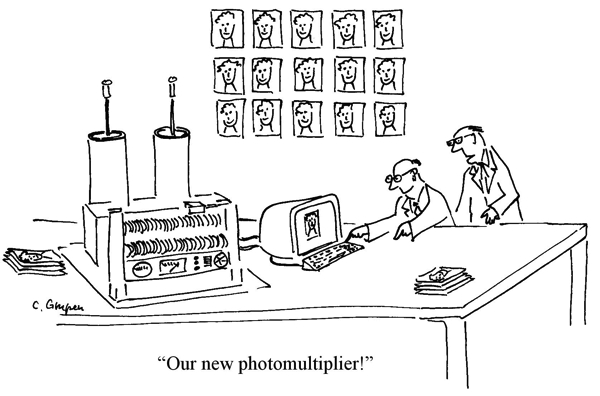
\includegraphics[scale=1]{fig14}
\end{center}
\end{frame}

\subsection{Diferencias estructurales}
\begin{frame}{Diferencias estructurales - I}
 
\begin{justify}
 Todos consisten de un fotocátodo semitransparente, una región de colección de fotoelectrones
 entre el fotocátodo y el primer dínodo, una sección de multiplicación de electrones 
 multietapa, y un ánodo para la colección de la carga amplificada. Estas estructuras están
 encerradas en una envoltura de vidrio al vacío, por la cual cables eléctricos son conducidos 
 en la base. (Les leeré un poquito sobre algunos tipos).
\end{justify}

\begin{figure}
\center
 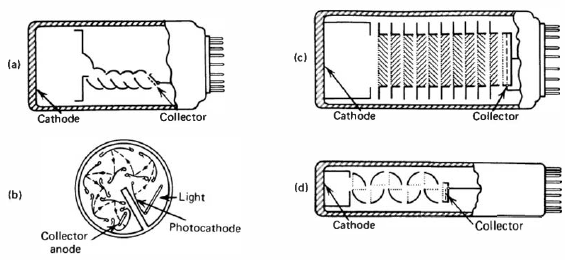
\includegraphics[scale=0.4]{fig15}
 \caption{\begin{footnotesize} Configuraciones para algunos tipos comunes de tubos FM. $(a)$ Estructura 
 lineal enfocada. $(b)$ Red circular. $(c)$ Persiana veneciana.
 $(d)$ Caja y red. \end{footnotesize}}
\end{figure}
 
\end{frame}

\begin{frame}{Diferencias estructurales - II}
\begin{columns}[c]
\column{2in}
 \begin{exampleblock}{Nota experimental}
  \begin{itemize}[<+->]
   \item \begin{justify}
          Los tubos con un plato plano de vidrio al final son los únicos tipos,
	  usados para conteo de centelladores.
         \end{justify}
   \item \begin{justify}
          Un diámetro de 5 cm es uno de las elecciones más comunes para aplicaciones 
          de centelleo.
         \end{justify}
   \item \begin{justify}
          Los tubos FM deben protegerse de vibraciones o choque mecánicos excesivos 
          para evitar un daño físico a los componentes internos.
         \end{justify}
  \end{itemize}
 \end{exampleblock}

  \column{2in}
  
  \begin{center}
 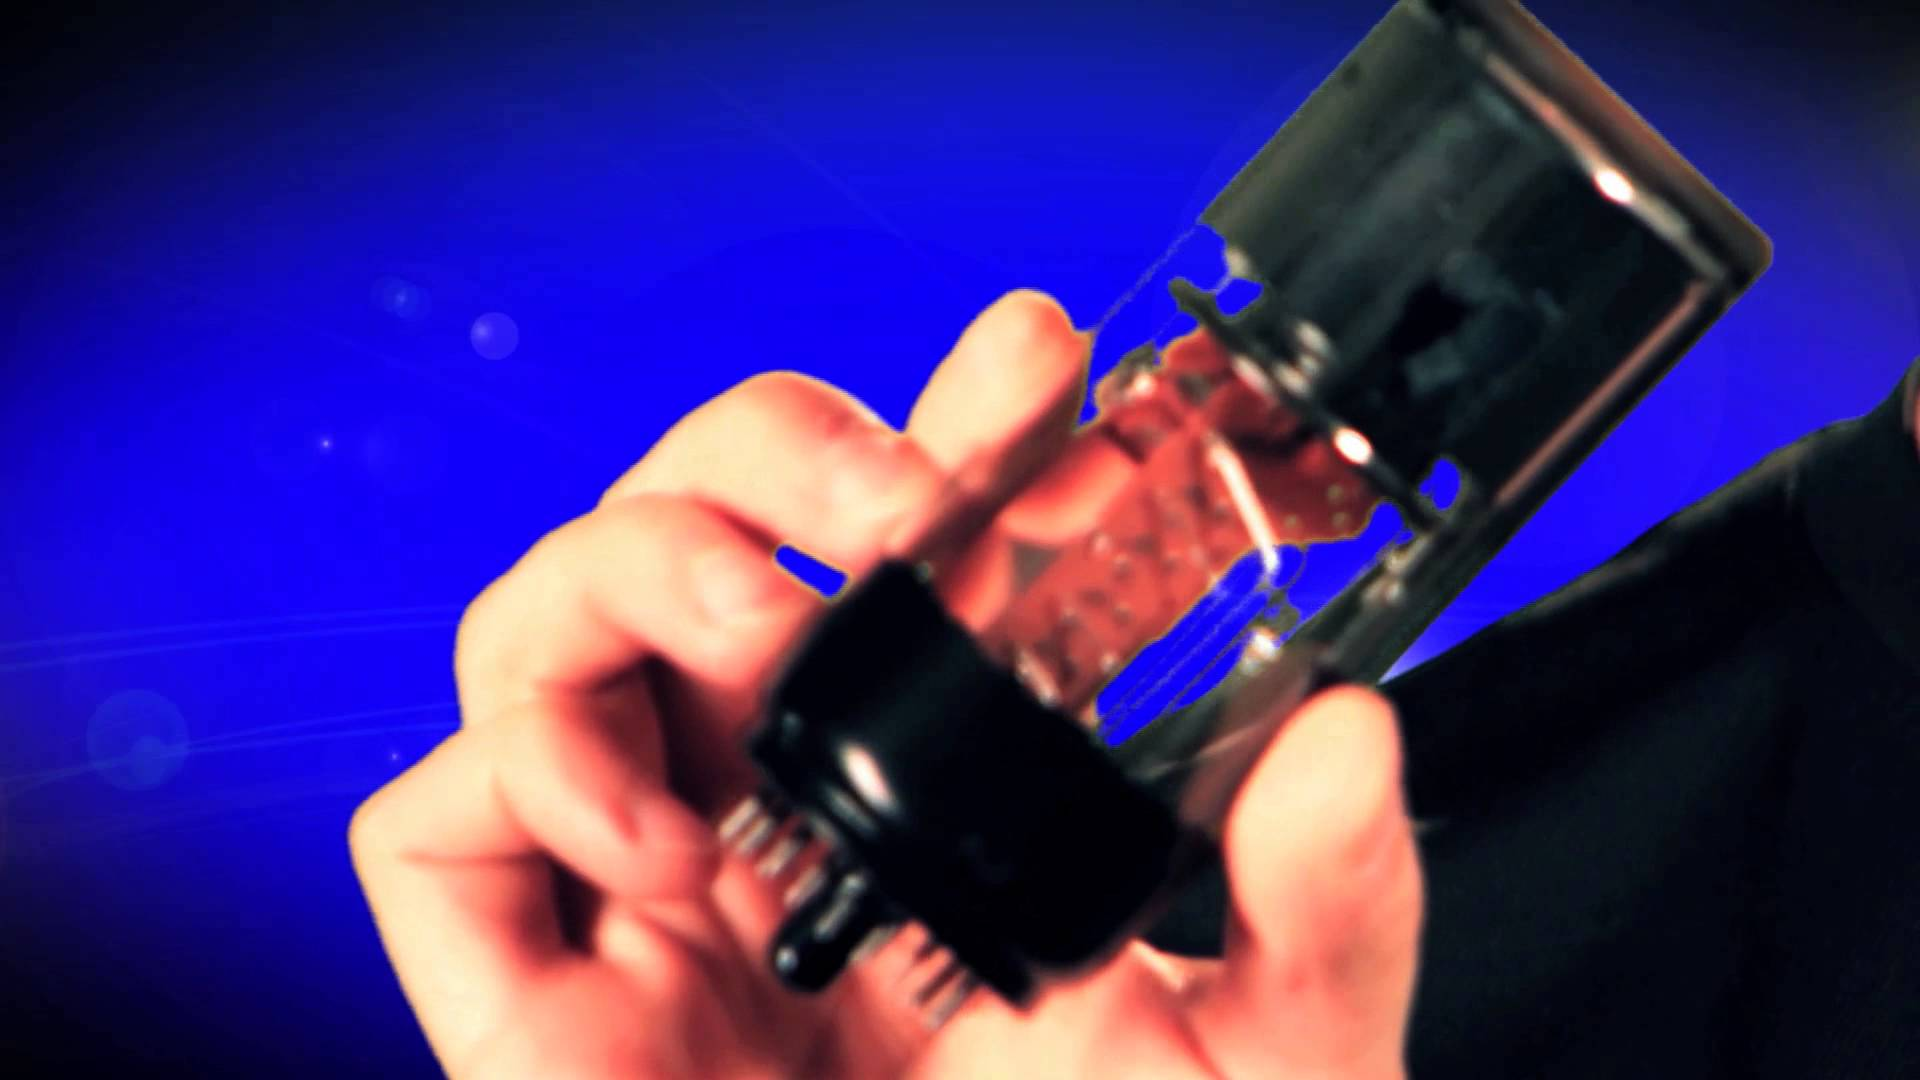
\includegraphics[scale=0.08]{fig22}
 \end{center}
  
  \end{columns}
\end{frame}

\begin{frame}{Diferencias estructurales - III}
 \begin{center}
  \Huge{\color{blue}Algunos tubos FM reales} \\
  \vspace{0.5cm}
 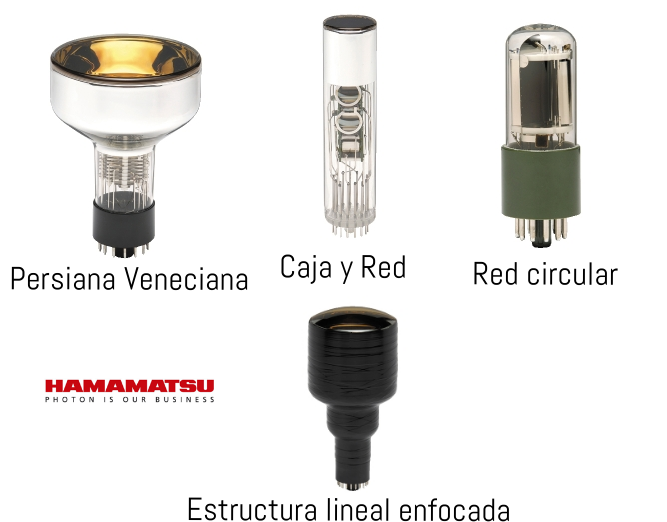
\includegraphics[scale=0.33]{fig21}
 \end{center}
\end{frame}

\subsection{Propiedades de temporización de pulsos}
\begin{frame}{Propiedades de temporización de pulsos - I}

\begin{justify}
Los tiempos característicos de un tubo FM están determinados exclusivamente 
por las trayectorias de electrones. El tiempo de tránsito de electrón de 
un tubo FM está definido por la diferencia de tiempo promedio entre la 
llegada de un fotón al fotocátodo y la colección de la subsecuente ráfaga 
de electrones en el ánodo.
\end{justify}

\begin{exampleblock}{Nota experimental}
 \begin{itemize} [<+->]
  \item \begin{justify}
         Los rangos de tiempo para el transito de electrón está entre los 
         $20-80$ ns. 
        \end{justify}
  \item \begin{justify}
         Sin embargo el tránsito solo no es de primaria importancia. El 
         esparcimiento del tiempo de tránsito es una cantidad más importante 
         porque determina la anchura de tiempo del pulso de electrones 
         que están llegando en el ánodo del tubo.
        \end{justify}
 \end{itemize}
\end{exampleblock}
 
\end{frame}

\begin{frame}{Propiedades de temporización de pulsos - II}
 
 \begin{columns}[c]
  \column{2in}
  
  \begin{figure}
  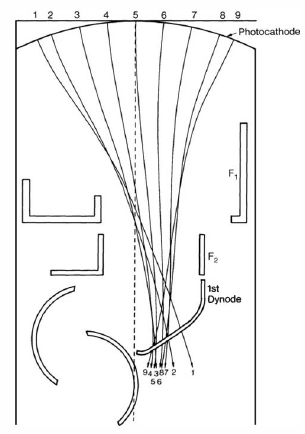
\includegraphics[scale=0.4]{fig23}
   \caption{Trayectorias generadas por computadora de los electrones 
   acelerados desde el fotocátodo al primer dínodo en un tubo FM.}
  \end{figure}
  
  \column{2.5in}
  \begin{exampleblock}{Nota experimental}
   \begin{itemize} [<+->]
    \item \begin{justify}
           La región entre el fotocátodo y el primer dínodo es crítica en 
           la determinación de las propiedades temporales. Para permitir 
           un colección uniforme sobre fotocátodos grandes, la distancia 
           entre ellos es considerablemente grande comparado con las distancias 
           entre dínodos.
          \end{justify}
    \item \begin{justify}
           La diferencia en los caminos entre un fotoelectrón que 
           deja el fotocátodo en el centro, y uno que lo deja en un 
           borde es un factor dominante en el esparcimiento observado 
           en el tiempo de tránsito.
          \end{justify}
   \end{itemize}

   
  \end{exampleblock}  
 \end{columns}

\end{frame}


\begin{frame}{Propiedades de temporización de pulsos - III}
 
 \begin{columns}[c]
  \column{2in}
  
  \begin{figure}
  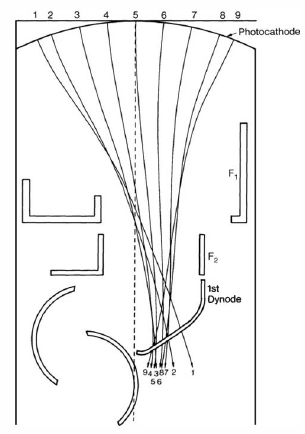
\includegraphics[scale=0.4]{fig23}
   \caption{Trayectorias generadas por computadora de los electrones 
   acelerados desde el fotocátodo al primer dínodo en un tubo FM.}
  \end{figure}
  
  \column{2.5in}
  \begin{exampleblock}{Nota experimental}
   \begin{itemize} [<+->]
    \item \begin{justify}
	  El fotocátodo usualmente es curvado para minimizar el esparcimiento 
	  del tiempo de tránsito a lo largo de su diámetro.
          \end{justify}
    \item \begin{justify}
          Una segunda fuente de esparcimiento de tiempo de tránsito surge de 
          la distribución inicial de velocidades de los fotoelectrones que 
          dejan el fotocátodo. Este efecto se puede minimizar usando una diferencia
          de voltaje más grande entre el fotocátodo y el primer dínodo.
          \end{justify}
   \end{itemize} 
  \end{exampleblock}  
 \end{columns}

\end{frame}

\begin{frame}{Propiedades de temporización de pulsos - IV}
 \begin{justify}

 Para simplificar el análisis y comparación entre diferentes fotomultiplicadores, 
 muchas de las mediciones reportadas en la literatura se concentran en el 
 esparcimiento de tiempo de tránsito debido a un sólo fotoelectrón. Por otra parte,
 si la distribución en los varios posibles esparcimientos en el tiempo de tránsito 
 se asumen gaussianos, la teoría estadística predice que el esparcimiento relativo
 en el tiempo de tránsito variará inversamente con la raíz cuadrada del número 
 de fotoelectrones.

 \end{justify}
 
 \begin{columns}[c]
  \column{2in}
  \begin{figure}
   \center 
   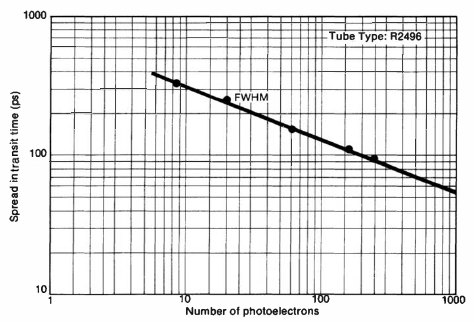
\includegraphics[scale=0.3]{fig24}
  \end{figure}
  
  \column{2in}
  \begin{block}{Nota relevante}
  \begin{justify}
   En la figura de la izquierda se verifica este comportamiento. Una alta producción 
   de luz de un centellador es importante en las aplicaciones de temporización, así 
   como en las mediciones de amplitud de pulso
   \end{justify}
  \end{block}
 \end{columns}

\end{frame}

\begin{frame}{Propiedades de temporización de pulsos - V}
\begin{exampleblock}{Nota experimental}
 \begin{justify}
 El esparcimiento temporal atribuible a la sección multiplicadora decrece con un 
 mayor voltaje entre dínodos, y el mejor desempeño en temporización normalmente es 
 obtenido operando el tubo al máximo voltaje permitido por los índices.
 
 \vspace{.3cm}
 
 Cuando se usan con centelladoras inorgánicas lentas, los tubos FM son lo suficientemente
 rápidos para que su contribución al tiempo total de respuesta usualmente no sea 
 un factor importante. Sólo cuando se emplean centelladoras con un tiempo de 
 decaimiento más bajo para derivar en una señal temporizadora rápida, que 
 los tubos FM se pueden convertir en un elemento significante en la determinación 
 de las propiedades de temporización resultantes.
 
 \end{justify}
\end{exampleblock}
 \end{frame}
 
\subsection{Índices máximos}
\begin{frame}{Índices máximos}

\begin{columns}[c]

\column{2in}
\begin{footnotesize}
\begin{justify}
Todos los tubos FM comerciales vienen con un conjunto de índices de voltajes máximos 
y corrientes máximas que no deben excederse durante el uso rutinario. Las especificaciones 
detalladas también darán valores individuales para los voltajes máximos entre 
el fotocátodo y el primer dínodo, dínodo a dínodo, del último dínodo al ánodo y 
del cátodo al ánodo.
\end{justify}
\end{footnotesize}

\begin{exampleblock}{Nota experimental}
\begin{justify}
 Debido a que virtualmente todos los tubos FM mostrarán un incremento en la ganancia 
 cuando el voltaje se aumenta, el valor máximo de voltaje aplicado prácticamente 
 determina la ganancia máxima que se puede obtener del tubo.
 \end{justify}
\end{exampleblock}

\column{2in}

\begin{figure}
 \center
 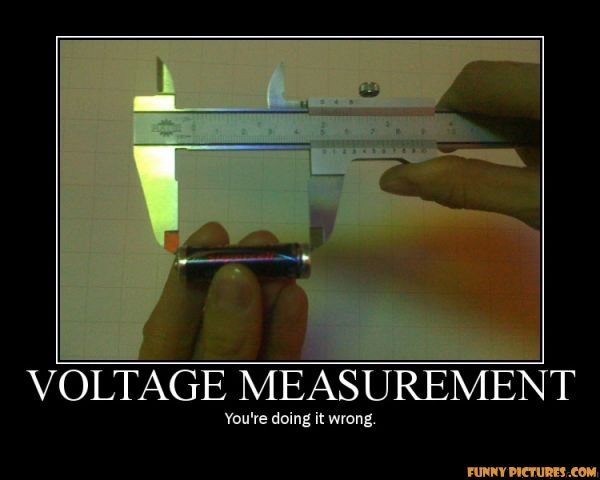
\includegraphics[scale=0.22]{fig25}
\end{figure}

\begin{figure}
 \center
 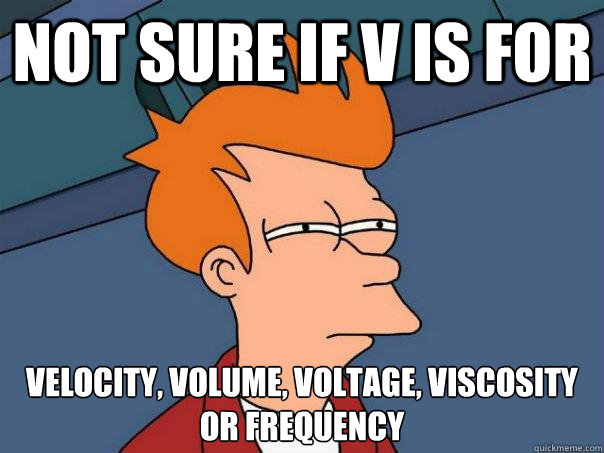
\includegraphics[scale=0.22]{fig26}
\end{figure}
\end{columns}

\end{frame}

\subsection{Especificaciones para tubos FM}
\begin{frame}{Especificaciones para tubos FM}

\begin{itemize}[<+->]
 \item \begin{justify}
        \textbf{Sensitividad luminosa total (A/lm)}: Razón entre la corriente medida en el
        ánodo a un voltaje de operación y el flujo luminoso de una fuente de luz de 
        tungsteno de temperatura especificada incidente en el fotocátodo.
       \end{justify}
 \item \begin{justify}
        \textbf{Sensitividad luminosa delc cátodo (A/lm)}: Definida como arriba, 
        excepto que la corriente de fotoelectrones que dejan el fotocátodo 
        es sustituida en el numerador por la corriente del ánodo.
       \end{justify}
 \item \begin{justify}
        \textbf{Sensitividad radiante total (A/W)}: Razón entre la corriente 
        del ánodo.
       \end{justify}
 \item \begin{justify}
        
       \end{justify}
 \item \begin{justify}
        
       \end{justify}
 \item \begin{justify}
        
       \end{justify}
\end{itemize}

 
\end{frame}





\end{document}
